\documentclass{beamer}
%
% Choose how your presentation looks.
%
% For more themes, color themes and font themes, see:
% http://deic.uab.es/~iblanes/beamer_gallery/index_by_theme.html
%
\mode<presentation>
{
  \usetheme{default}      % or try Darmstadt, Madrid, Warsaw, ...
  \usecolortheme{default} % or try albatross, beaver, crane, ...
  \usefonttheme{default}  % or try serif, structurebold, ...
  \setbeamertemplate{navigation symbols}{}
  \setbeamertemplate{caption}[numbered]
} 

\usepackage[spanish]{babel}
\usepackage[utf8x]{inputenc}


\title[Clase 4]{Procesamiento de bases de datos con STATA}
\subtitle{Clase 4}
\author{Claudia Vazquez}
\date[]{\texttt{clauvazqu@gmail.com}Centro REDES}
\pgfdeclareimage[height=0.5cm]{university-logo}{logo-redes}
\logo{\pgfuseimage{university-logo}}

\begin{document}

\begin{frame}
  \titlepage
\end{frame}

\begin{frame}{Contenido}
  \tableofcontents
 \end{frame}


\section{archivos log y do}
\subsection{log}
\begin{frame}{Archivos log}
\begin{itemize}
\item Es importante tener una ``memoria'' de la sesión de trabajo. STATA guarda nuestra sesión de trabajo en un archivo llamado ``log'', pero no lo hace automáticamente.
\item El comando para crear un log es:\\ {\footnotesize \texttt{log using \textit{filename}, replace}}
\item El archivo ``log'' guarda los comandos ejecutados y los resultados de la ventana ``Results''.
\item A partir de ese momento, se guarda el registro de todo lo que hagamos.
\item La opción \texttt{replace} implica que los resultados se sobre-escriben. 
\end{itemize}
\end{frame}

\begin{frame}{Comandos para crear un log}
\begin{itemize}
\item El comando \texttt{log using} da error si ya tenemos un log abierto: para crear un log debemos primero cerrar cualqueir otro abierto.
\item El comando para cerrar un log es \texttt{log close}.
\item El problema es que el comando \texttt{log close} da error si \textbf{no} hay un log en uso.
\item Para evitar que nos de error en los archivos do que veremos a continuación anteponemos el comando \texttt{capture}, que suprime todo el output, incluyendo los mensajes de error.
\end{itemize}
\end{frame}

\subsection{do}
\begin{frame}[allowframebreaks]{Archivos do}
\begin{itemize}

\item Hasta ahora, la interacción con STATA ha sido mediante el tipeo de comandos en la ventana ``Command'.
\item En vez de ir tipeando cada comando, se puede crear un archivo de texto y decirle a STATA que ejecute secuencialmente todos los comandos almacenados en ese archivo. 
\item Estos archivos se llaman \textit{do-file} porque el comando que los ejecuta es \texttt{do}.
\item Es posible editarlos con el editor de STATA, al que se accede mediante el comando \texttt{doedit}, o con editores externos como Editplus (\url{www.editplus.com}).
\item Trabajar con \textit{do-files} tiene muchas ventajas. Entre otras: 

\begin{itemize}
\item Al escribir los comandos utilizados para procesar y analizar una base de datos, nos queda un registro de lo que hemos hecho y el trabajo se puede reproducir en otro momento.
\item Si decidimos cambiar una parte del análisis, modificamos los comandos necesarios en el \textit{do-file} y no tenemos que empezar todo de nuevo, como cuando trabajamos interactivamente.
\end{itemize}

\item Para crear un archivo do abrimos el editor, escribimos las sentencias que se desean ejecutar y guardamos el archivo en nuestra carpeta de trabajo con extensión .do (si usamos el editor de STATA esta extensión viene por defecto).

\item Supongamos que usamos el editor de STATA para crear un archivo llamado trabajo.do que contiene estas tres líneas:\\
\rule{11cm}{0.1pt}\\
{\footnotesize
\texttt{use http://www.stata-press.com/data/r12/census5}\\
\texttt{tabulate region}\\
\texttt{summarize marriage\_rate if state!=``Nevada''}}\\
\rule{11cm}{0.1pt}\\
\item Luego, nos ubicamos en nuestra carpeta de trabajo (la misma donde está guardado el archivo) y desde la línea de comando escribimos \texttt{do trabajo}. El resultado es el siguiente:
\end{itemize}
\centerline{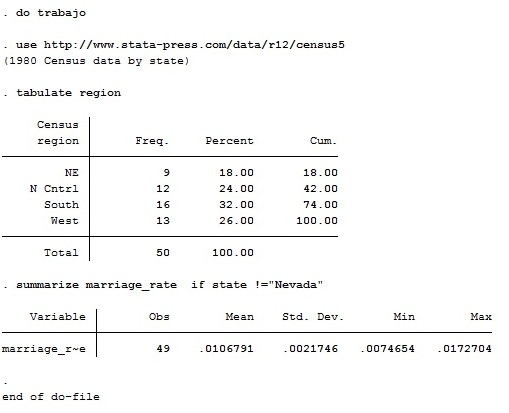
\includegraphics[height=6.5cm]{fig1.jpg}}
\begin{itemize}
\item Se recomienda que la primera línea en el \textit{do-file} declare la versión de STATA que se usó al momento de escribir el archivo, así nos aseguramos que el código va a funcionará si se corre en una versión posterior. El comando para hacerlo es \texttt{version}.
\item En los \textit{do-file} pueden introducirse comentarios: frases que STATA ignora pero que facilitan el entendimiento del código.
\item Se consideran comentarios las líneas que empiezan con asterisco (*), doble barra (//) o un bloque encerrado entre /* y */.
\item Si una sentencia es demasiado larga se puede separar en dos o más líneas con /// 
\item El comando \texttt{set more off} le dice a STATA que no muestre el mensaje ----\texttt{more}---- y que por lo tanto no haga una pausa en cada pantalla. Se recomienda que siempre forme parte del encabezado de los archivos do.
\item También se recomienda que los archivos do creen siempre un archivo log para almacenar todos los resultados. 
\item La ejecución del archivo do se interrumpe cuando ocurre un error.
\item Si nosotros deseamos detener la ejecución del do voluntariamente podemos aprentar el botón de \textit{break} en el menú: 
\includegraphics[height=0.35cm]{break.jpg}
\item Dentro de los do-files pueden ejecutarse otros archivos do (STATA permite hasta 64 niveles de profundidad).
\end{itemize}
\end{frame}

\begin{frame}{Ejemplo de un archivo do}
\centerline{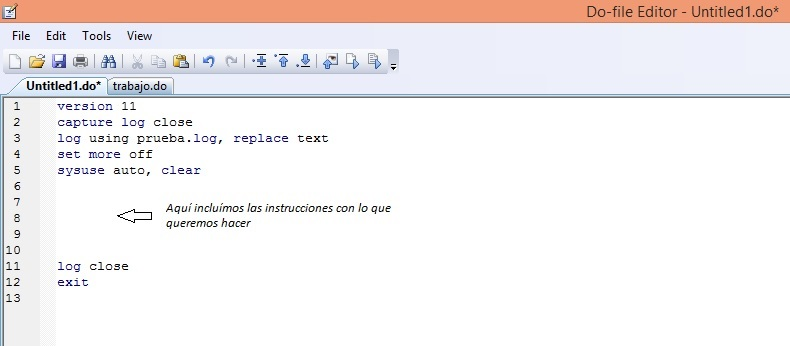
\includegraphics[height=5cm]{do.jpg}}
\end{frame}

\section{Gestión avanzada de bases de datos}
\subsection{xpose}

\begin{frame}[allowframebreaks]{xpose}
\begin{itemize}
\item El comando \texttt{xpose} permite transponer una base de datos, cambiando variables por observaciones y observaciones por variables.
\item Como ejemplo, cargamos una de las bases de datos de STATA que contiene información por país y año: \\\medskip
{\footnotesize \texttt{use http://www.stata-press.com/data/r12/xposexmpl}\\
\texttt{list}}\\\medskip
\centerline{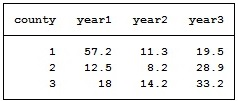
\includegraphics[height=2cm]{xpose.jpg}}
\item Para trasponerla y que cada observación refleje un año, escribimos:\\\medskip
{\footnotesize \texttt{xpose, clear varname}\\
\texttt{list}}\\
\centerline{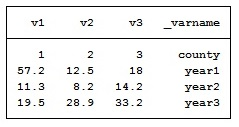
\includegraphics[height=2.5cm]{xpose1.jpg}}
\item Ahora debemos eliminar la primer observación (que corresponde a la antigua variable ``country'').
\end{itemize}
\end{frame}

\subsection{reshape}
\begin{frame}[allowframebreaks]{reshape}
\begin{itemize}
\item El comando \texttt{reshape} permite reestructurar la base de datos, alternando entre dos configuraciones llamadas \textit{wide} y \textit{long}.
\item La forma \textit{wide} guarda los datos de una observación en una fila, mientras que en la forma \textit{long} una observación corresponde a más de una fila: 
\end{itemize}
\centerline{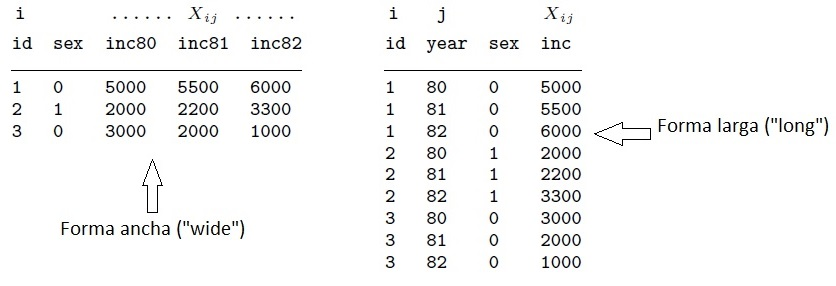
\includegraphics[height=3.3cm]{graf3.jpg}}
\begin{itemize}
\item En el ejemplo, en la base de la izquierda la variable ``id'' identifica al individuo y las variables ``inc80'', ``inc81'' y ``inc82'' representan el ingreso en los años 80, 81 y 82 respectivamente.
\item En la base de la derecha, la información es la misma pero se agrega la variable ``year'' y las variables de ingreso se transforman en una sola (``inc'').
\item Antes de usar el comando \texttt{reshape} debemos determinar si nuestro datos tienen forma \textit{wide} o \textit{long}.
\item Tambien cuál es la observación lógica ($i$) y la subobservación ($j$) a partir de las cuales se reorganizarán los datos.
\item En el ejemplo, para pasar de una forma a otra usamos los comandos:
\begin{itemize}
\item {\footnotesize \texttt{reshape long inc, i(id) j(year)}} \hspace{0.05cm} $\rightarrow$ {\footnotesize pasa de \textit{wide} a \textit{long}}
\item {\footnotesize \texttt{reshape wide inc, i(id) j(year)}} \hspace{0.05cm} $\rightarrow$ {\footnotesize pasa de \textit{long} a \textit{wide}}
\end{itemize}
\item Como no especificamos la variable ``sex'' STATA asume que es constante a lo largo de la variable ``id''.
\item Para comprender la utilidad de este comando debe tenerse en cuenta que las operaciones a lo largo de variables (columnas) son una cosa y las operaciones a través de observaciones (a lo largo de filas) son otras y \underline{no son igualmente fáciles} de implementar.
\end{itemize}
\end{frame}

\subsection{collapse}

\begin{frame}[allowframebreaks]{collapse}
\begin{itemize}
\item El comando \texttt{collapse} crea, a partir de la base de datos en memoria, una base que contiene estadísticas de resumen (promedios, sumas, etc.).
\item Hay que tener cuidado porque este comando destruye los datos originales.
\item Usamos como ejemplo la base empresas.dta, que tiene información ficticia sobre las ventas totales y el empleo para un conjunto de empresas en el periodo 2000-2003: \\\medskip
{\footnotesize 
\texttt{use empresa,clear}\\
\texttt{list}}\\\medskip
\centerline{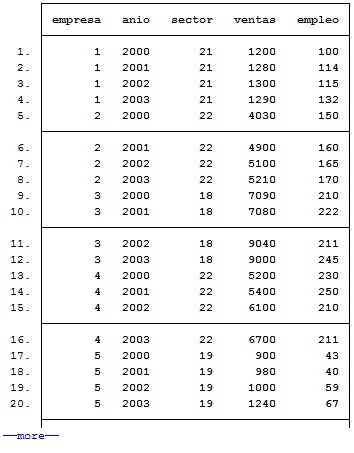
\includegraphics[height=5.3cm]{emp.jpg}}
\item Si quisiéramos tener una base con las ventas totales y el empleo promedio \underline{por sector de actividad}, hacemos:\\\medskip
{\footnotesize 
\texttt{collapse (sum) ventas (mean) empleo, by(sector)}\\
\texttt{list}}\\\medskip
\centerline{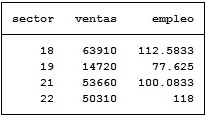
\includegraphics[height=2cm]{emp1.jpg}}
\item Después del \texttt{collpse}, primero se especifica el estadístico entre paréntesis y después la \textit{varlist}. 
\item En este caso, la \textit{varlist} se refiere exclusivamente a variables numéricas. 
\item La variable en el by() puede ser \textit{string} o numérica.
\end{itemize}
\end{frame}
\end{document}


QUEDÓ PENDIENTE: 
Actualización de stata


\begin{frame}
\begin{itemize}
\item Veamos cómo se pueden detectar y eliminar observaciones duplicadas
\item Cargamos en memoria el auto.dta que, como sabemos, tiene 74 observaciones
\item Crearemos 3 observaciones repetidas usando el comando ``expand exp'' que copia observaciones
\end{itemize}
\bigskip
\includegraphics[height=3cm]{ejemplo1.jpg}
\end{frame}

\begin{frame}{}
\begin{itemize}
\item Ahora detectaremos esas observaciones repetidas, para lo cual usamos el [by varlist:] con la lista completa de variables \\
\textbf{bysort} \_all : \textbf{gen} repite = \_N
\item Si todas las observaciones son distintas se armaran grupos conteniendo una sola observación cada uno:\\
\includegraphics[height=4.2cm]{ejemplo3.jpg}
\item Podemos eliminar los repetidos con el comando \textbf{duplicates drop}
\end{itemize}
\end{frame}

Indicator values for levels of factor variables
